\documentclass{article}

\usepackage{natbib}
\usepackage[sc]{mathpazo}
\usepackage[T1]{fontenc}
\usepackage{amsmath}
\usepackage{amsfonts}
\usepackage{amssymb}
\usepackage{graphicx}
\usepackage[onehalfspacing]{setspace}
\usepackage{color}
\usepackage[margin=.75in, tmargin=0.71in, bmargin=0.71in]{geometry}
\usepackage{url}

\usepackage{appendix}
\usepackage{hyperref}
\usepackage{xcolor}
\usepackage{todonotes}
\usepackage{booktabs}
\usepackage{lscape}
\usepackage{caption}%
\usepackage{bbm}
\usepackage{comment}

\usepackage{longtable}

\usepackage{subcaption}

\usepackage{babel}
\usepackage[autostyle, english = american]{csquotes}
\MakeOuterQuote{"}

\title{Textual Analysis and Financial Statements}
\author{Isaac Liu}

\setlength{\parindent}{0pt}
\setlength{\parskip}{0.5em}

\hypersetup{
    colorlinks=true,
    linkcolor=black,
    filecolor=black,      
    urlcolor=blue,
    citecolor=black
}

\begin{document}

	\maketitle

    \section*{Introduction}

    note credit rating data access is limited and our model can be used to interpolate
    
    \section*{Data}

    \citep{das_credit_2023}

	\begin{figure}[h!]
		\centering
        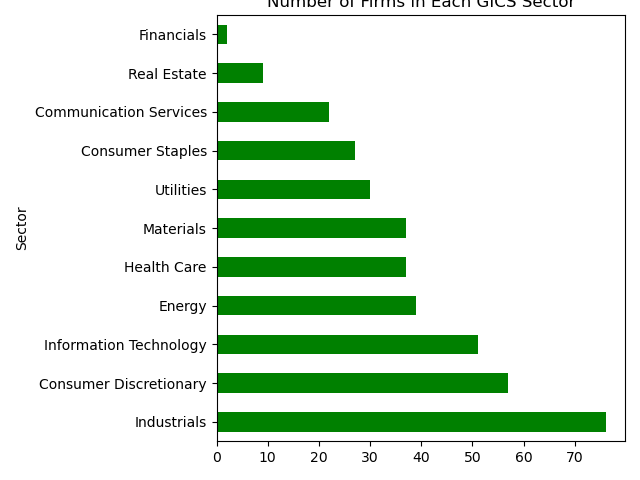
\includegraphics[width=\linewidth,keepaspectratio=true]{../Output/all_data_fixed_quarter_dates_firms_by_sector.png}
	\end{figure}
    
    \section*{Conclusion}

    Overall, there may be some merit to current arguments suggesting the presence of political costs and benefits of welfare-enhancing commitment institutions such as central bank independence and fixed exchange rates. This suggests some role for the political economy analysis of the choice of these institutions.
    
    \clearpage
    \newpage

    \bibliographystyle{chicago}
    \bibliography{Stat-222-Capstone}

    \clearpage
    \newpage

    \appendix

    \section*{Appendix}

\end{document}
